\chapter{Versuchsaufbau}
    Mit LT-Spice ist ein stromgegengekoppelter Verstärker in Emitterschaltung aufgebaut.
    \begin{figure}[h!]
        \centering
        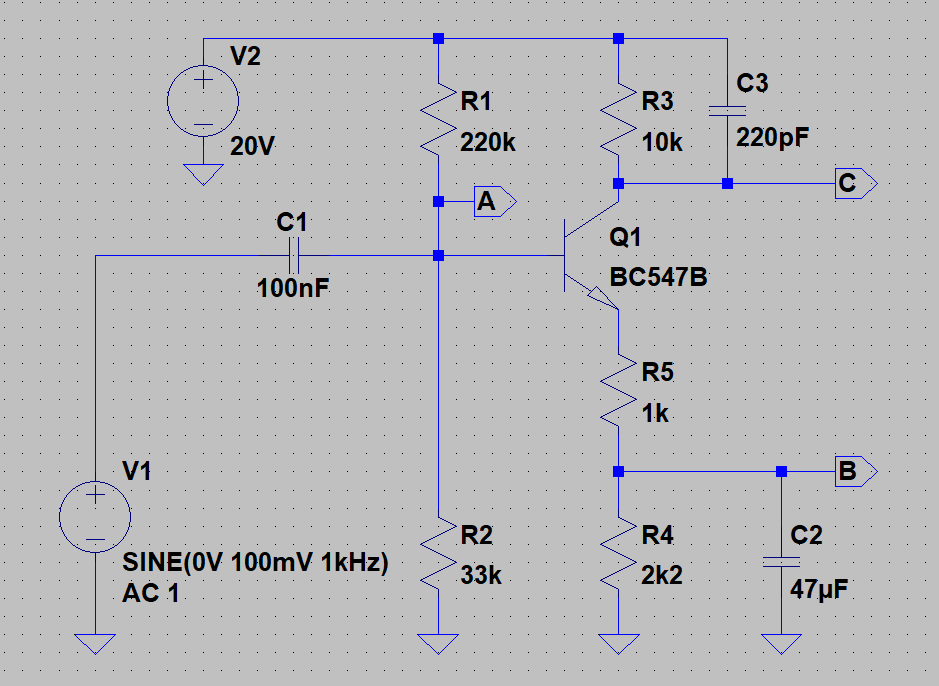
\includegraphics[width=0.7\linewidth]{2.PNG}
        \caption{Aufbau eines stromgegengekoppelten Verstärkers in Emitterschaltung}
    \end{figure}

    Die Schaltung ist aus verschiedenen Widerständen R, Kondensatoren C und Ausgängen (A,B,C) aufgebaut. Hinzu kommt eine Wechselspannung V1 und eine Gleichspannung V2. In der Schaltung ist auch der Transistor Q1 verbaut.